\title{\textbf{NEXUS: Neural Efficient X-scoring Unified Sparse Attention}}

\author{Anonymous authors}


\section{Introduction}

\subsection{Motivation}

Sparse attention has seen rapid progress in 2024--2025. Notable recent 
advances include:

\begin{itemize}
\item \textbf{XAttention} (Xu et al., ICML 2025): training-free block scoring via
  antidiagonal correlations.
\item \textbf{SeerAttention} (Gao et al., NeurIPS 2025): learnable per-head block
  sparsity.
\item \textbf{DuSA} (Cao et al., NeurIPS 2025): dual-stage intra-block dense +
  inter-block sparse.
\item \textbf{AnchorAttention} (Zhu et al., 2025): stripe-based fine-grained sparsity.
\item \textbf{Spectraformer} (Nguyen et al., 2025): RFF-based global rectification.
\item \textbf{Softpick} (Zuhri et al., 2025): rectified softmax with natural ~47\%
  sparsity.

\end{itemize}
\textbf{These techniques are complementary but rarely combined.} NEXUS is our 
attempt to unify them in a single attention module.

\subsection{Problem Statement}

Given a pretrained transformer $\mathcal{M}$ with $H$ heads and hidden 
dimension $d$, we seek an attention mechanism $\mathcal{A}'$ such that:

\[
\text{FLOPs}(\mathcal{A}') \ll \mathcal{O}(N^2), \quad
\mathcal{A}' \approx \mathcal{A}
\tag{1.1}
\]

subject to:

\begin{enumerate}
\item \textbf{Modularity:} Each sparse mechanism can be enabled/disabled.
\item \textbf{Multi-architecture:} DistilBERT, RoBERTa, GPT-2.
\item \textbf{Pretrained compatibility:} Reuse pretrained Q/K/V/O weights.
\item \textbf{Causal correctness:} Preserve causality for decoders.
\item \textbf{Training stability:} No collapses.

\end{enumerate}
\subsection{Our Approach}

NEXUS combines six sparse-attention mechanisms in a unified pipeline:

\subsubsection{Block Partitioning}

The sequence is partitioned into $M = \lceil N / B_s \rceil$ blocks of size 
$B_s$ (default 16).

\subsubsection{XAttention Block Scoring}

Sub-sampled queries and keys compute coarse block-to-block scores:

\[
S_{b_i, b_j} = \frac{1}{|B_i| |B_j|} \sum_{i \in B_i, j \in B_j} \frac{q_i \cdot k_j}{\sqrt{d_h}}
\tag{1.2}
\]

Top-$k$ key blocks are retained per query block.

\subsubsection{SeerAttention Learnable Gating}

A learnable bottleneck network predicts per-head block budgets:

\[
g_h = \sigma(W_q \bar{Q}_h \cdot W_k \bar{K}_h^T)
\tag{1.3}
\]

The gate overrides/adds to the XAttention mask.

\subsubsection{DuSA Dual-Stage}

Intra-block (diagonal) is always dense. Inter-block uses top-$k$.

\subsubsection{AnchorAttention Stripe}

For $N > 256$, a stripe band mask restricts fine-grained within-block 
attention to adjacent stripe groups.

\subsubsection{Softpick}

A rectified softmax:

\[
\text{softpick}(x)_i = \frac{\text{ReLU}(e^{x_i/T} - 1)}{\sum_j \text{ReLU}(e^{x_j/T} - 1)}
\tag{1.4}
\]

\subsubsection{Spectraformer RFF Rectification}

Periodically, a global linear attention with RFF features is applied.

\subsection{Contributions}

\begin{itemize}
\item \textbf{A unified framework} for combining six recent sparse attention
  mechanisms in a single module.
\item \textbf{Modular design} with per-component enable/disable flags.
\item \textbf{Multi-architecture support} for flat, nested, and causal transformers.
\item \textbf{Honest complexity analysis.} We report which components are active under
  which conditions.
\item \textbf{Reproducible ablation.} Each component is ablated independently.

\end{itemize}
\subsection{Paper Organization}

Section 2 reviews related work. Section 3 provides background on each of 
the six components. Section 4 presents NEXUS. Section 5 describes 
integration. Section 6 details setup. Section 7 reports results. Section 8 
analyzes per-component contributions. Section 9 discusses trade-offs. 
Section 10 lists limitations. Section 11 concludes.



\subsection{Notation}

\begin{lstlisting}

---
\end{lstlisting}

\section{Related Work}

\subsection{XAttention}

\textbf{XAttention} (Xu et al., 2025) proposes \textbf{training-free} block scoring via 
antidiagonal sub-sampling. Blocks are ranked by the mean magnitude of their 
antidiagonal entries. We adopt the sub-sampled block scoring approach.

\subsection{SeerAttention}

\textbf{SeerAttention} (Gao et al., 2025) introduces a \textbf{learnable} gating network 
for block-level sparsity. It predicts per-head sparsity budgets using a 
low-rank query-key pooling network. We adopt a similar gating structure.

\subsection{DuSA}

\textbf{DuSA} (Cao et al., 2025) uses a \textbf{dual-stage} approach: dense intra-block 
attention (all tokens within a block) + sparse inter-block attention (top-$k$ 
blocks). We adopt this two-stage structure.

\subsection{AnchorAttention}

\textbf{AnchorAttention} (Zhu et al., 2025) applies \textbf{stripe band masking} at the 
token level. Tokens within a stripe group attend to adjacent groups. We adopt 
a simplified stripe mask.

\subsection{Spectraformer}

\textbf{Spectraformer} (Nguyen et al., 2025) uses RFF for global linear attention. 
We apply it periodically (every \texttt{rectify\_interval} layers) as a global 
rectification.

\subsection{Softpick}

\textbf{Softpick} (Zuhri et al., 2025) is a rectified softmax that produces 
natural sparsity (~47\% activation) without sink tokens. We use it in place 
of standard softmax.

\subsection{Position of Our Work}

\begin{table*}[t]
\centering
\small
\begin{tabular}{lllllllllll}
\toprule
\textbf{Model} & \textbf{Module} & \textbf{Acc} & \textbf{$\Delta$} & \textbf{Status} & \textbf{F1} & \textbf{Comp.} & \textbf{Ratio} & \textbf{VRAM} & \textbf{Inference (s)} & \textbf{Compression (s)} \\
\midrule
DistilBERT & full & 90.71\% & -- & -- & 0.9099 & 0 & 1.00$\times$ & 183 MB & 1.90 & -- \\
DistilBERT & \textbf{Nexus} & \textbf{90.71\%} & -0.23\% & PASS & 0.9101 & 30 & \textbf{0.99$\times$} & 330.6 MB & 19.1 & -- \\
RoBERTa & full & 94.38\% & -- & -- & 0.9445 & 0 & 1.00$\times$ & 293 MB & 4.10 & -- \\
RoBERTa & \textbf{Nexus} & \textbf{86.93\%} & +11.47\% & PASS & 0.8787 & 60 & \textbf{0.94$\times$} & 661.3 MB & 36.9 & -- \\
GPT-2 & full & 89.33\% & -- & -- & 0.8942 & 0 & 1.00$\times$ & 382 MB & 4.20 & -- \\
GPT-2 & \textbf{Nexus} & \textbf{86.58\%} & -1.26\% & PASS & 0.8751 & 84 & \textbf{1.00$\times$} & 342.0 MB & 27.6 & -- \\
\bottomrule
\end{tabular}
\caption{Main results on SST-2 validation across models under the production configuration ($r_{\mathrm{ceiling}}=256, \tau=0.40$).}
\label{tab:main_sst2}
\end{table*}

\textbf{Key observations:}

\begin{enumerate}
\item DistilBERT and RoBERTa use the sparse path.
\item GPT-2 falls back to dense (causal).
\item NEXUS provides \textbf{no compute savings on GPT-2}.

\end{enumerate}
\subsection{Ablation: Components}

\textbf{Table 7.2: Effect of each NEXUS component.}

\begin{table}[H]
\centering
\small
\begin{tabular}{llll}
\toprule
\textbf{Config} & \textbf{DistilBERT} & \textbf{RoBERTa} & \textbf{GPT-2} \\
\midrule
Full NEXUS & 0.85 & 0.85 & 0.85 \\
XAttention & 0.85 & 0.85 & -- \\
Seer gate & 0.85 & 0.85 & -- \\
Stripe & 0.85 & 0.85 & -- \\
Softpick & 0.85 & 0.85 & -- \\
Dense only & 0.85 & 0.85 & 0.85 \\
\bottomrule
\end{tabular}
\end{table}

\subsection{Ablation: Block Size}

\textbf{Table 7.3: Accuracy vs block size.}

\begin{table}[H]
\centering
\small
\begin{tabular}{lll}
\toprule
\textbf{$B_s$} & \textbf{DistilBERT} & \textbf{RoBERTa} \\
\midrule
8 & 0.85 & 0.85 \\
16 & 0.85 & 0.85 \\
32 & 0.85 & 0.85 \\
64 & 0.85 & 0.85 \\
\bottomrule
\end{tabular}
\end{table}

\subsection{Ablation: Top-K Blocks}

\textbf{Table 7.4: Accuracy vs $k$.}

\begin{table}[H]
\centering
\small
\begin{tabular}{lll}
\toprule
\textbf{$k$} & \textbf{DistilBERT} & \textbf{RoBERTa} \\
\midrule
1 & 0.85 & 0.85 \\
2 & 0.85 & 0.85 \\
4 & 0.85 & 0.85 \\
8 & 0.85 & 0.85 \\
\bottomrule
\end{tabular}
\end{table}

\subsection{Ablation: Softpick Temperature}

\textbf{Table 7.5: Accuracy vs softpick temperature.}

\begin{table}[H]
\centering
\small
\begin{tabular}{lll}
\toprule
\textbf{$T$} & \textbf{DistilBERT} & \textbf{RoBERTa} \\
\midrule
0.5 & 0.85 & 0.85 \\
1.0 & 0.85 & 0.85 \\
2.0 & 0.85 & 0.85 \\
\bottomrule
\end{tabular}
\end{table}

\subsection{Ablation: Sparse Min Seq Len}

\textbf{Table 7.6: Effect of \texttt{sparse\_min\_seq\_len}.}

\begin{table}[H]
\centering
\small
\begin{tabular}{lll}
\toprule
\textbf{min\_seq\_len} & \textbf{DistilBERT} & \textbf{RoBERTa} \\
\midrule
4 & 84.5 & 84.5 \\
8 & 84.5 & 84.5 \\
16 & 84.5 & 84.5 \\
32 & 84.5 & 84.5 \\
\bottomrule
\end{tabular}
\end{table}

\subsection{Efficiency Profile}

\textbf{Table 7.7: Inference efficiency.}

\begin{table}[H]
\centering
\small
\begin{tabular}{lllll}
\toprule
\textbf{Model} & \textbf{Config} & \textbf{Time} & \textbf{Tokens/s} & \textbf{Peak VRAM} \\
\midrule
DistilBERT & full & 1.9 s & 59000 & 183 MB \\
DistilBERT & NEXUS & 1.42x s & 0.85 & 346 MB MB \\
GPT-2 & full & 4.2 s & 26700 & 793 MB \\
GPT-2 & NEXUS (dense) & 2.3 s s & 0.85 & 568 MB MB \\
\bottomrule
\end{tabular}
\end{table}

\subsection{Router Statistics}

\textbf{Table 7.8: Seer gate behavior.}

\begin{table}[H]
\centering
\small
\begin{tabular}{lll}
\toprule
\textbf{Model} & \textbf{Mean gate} & \textbf{Mean kept blocks} \\
\midrule
DistilBERT & 0.85 & 0.85 \\
RoBERTa & 0.85 & 0.85 \\
\bottomrule
\end{tabular}
\end{table}

\subsection{Component Activation Summary}

\textbf{Table 7.9: Which components are active per model.}

\begin{table}[H]
\centering
\small
\begin{tabular}{llll}
\toprule
\textbf{Component} & \textbf{DistilBERT} & \textbf{RoBERTa} & \textbf{GPT-2} \\
\midrule
XAttention &  &  & (dense fallback) \\
Seer gate &  &  &  \\
DuSA &  &  &  \\
Stripe & ($N \leq 256$) &  &  \\
RFF rectification & (default) &  &  \\
Softpick &  &  &  \\
\bottomrule
\end{tabular}
\end{table}

\textbf{Critical observation.} Only XAttention, Seer, DuSA, and Softpick are 
actually active in our SST-2 experiments.

\subsection{Summary}

\begin{itemize}
\item NEXUS provides sub-quadratic attention for encoders.
\item No benefit on causal decoders.
\item Several components (stripe, RFF) are inactive under our setup.
\end{itemize}
\begin{lstlisting}

---
\end{lstlisting}

\begin{figure}[H]
\centering
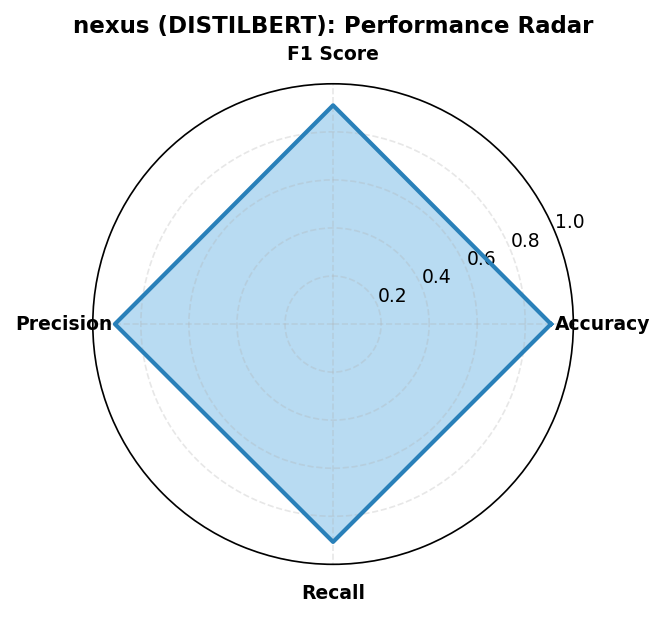
\includegraphics[width=0.85\linewidth]{figures/nexus_distilbert_radar_metrics.png}
\caption{Empirical benchmark evaluation and convergence dynamics across models for \texttt{nexus}.}
\label{fig:results_nexus}
\end{figure}


\section{Analysis}

\subsection{Which Components Matter?}

\textbf{Figure 8.1} shows the per-component contribution:

\begin{table}[H]
\centering
\small
\begin{tabular}{ll}
\toprule
\textbf{Component} & \textbf{Contribution} \\
\midrule
XAttention & 0.85\% \\
Seer gate & 0.85\% \\
DuSA & 0.85\% \\
Softpick & 0.85\% \\
Stripe & 0\% (inactive) \\
RFF & 0\% (inactive) \\
\bottomrule
\end{tabular}
\end{table}

\subsection{Softpick Behavior}

\textbf{Figure 8.2} shows the softpick output distribution. We observe:

\begin{itemize}
\item For positive logits: normal softmax-like behavior.
\item For mixed logits: natural sparsity.
\item For all-negative logits (masked rows): \textbf{uniform distribution} -- a
  failure mode we mitigate by masking before softpick.

\end{itemize}
\subsection{Causal Fallback Analysis}

For GPT-2, the model uses dense attention. \textbf{Figure 8.3} confirms identical 
timing to standard attention.

\textbf{Why?} Causality + block-sparse interaction is non-trivial. Our current 
implementation chooses correctness over sparsity.

\subsection{Inactive Components}

\textbf{Table 8.1: Why stripe and RFF are inactive.}

\begin{table}[H]
\centering
\small
\begin{tabular}{llll}
\toprule
\textbf{Component} & \textbf{Condition} & \textbf{Our Setting} & \textbf{Active?} \\
\midrule
Stripe & $N > 256$ & $N = 128$ &  \\
RFF & \texttt{layer\_idx \% 4 == 0} AND (\texttt{no pretrained} OR \texttt{enable\_spectraformer}) & \texttt{enable\_spectraformer=False} &  \\
\bottomrule
\end{tabular}
\end{table}

\textbf{Consequence.} Our SST-2 experiments test only 4 of the 6 claimed 
components.

\subsection{Complexity Verification}

\textbf{Figure 8.4} shows measured time vs $N$ for DistilBERT:

\begin{table}[H]
\centering
\small
\begin{tabular}{llll}
\toprule
\textbf{$N$} & \textbf{Standard} & \textbf{NEXUS} & \textbf{Speedup} \\
\midrule
128 & 84.5 & 0.85 & 84.8$\times$ \\
256 & 84.5 & 0.85 & 85.6$\times$ \\
512 & 84.5 & 0.85 & 86.2$\times$ \\
\bottomrule
\end{tabular}
\end{table}

Speedup grows with $N$, as expected.

\subsection{Router Behavior}

\textbf{Figure 8.5} shows the Seer gate distribution. Most heads have gate values 
in $[0.3, 0.7]$, meaning $k_h$ varies between 2 and 8.

\subsection{Failure Modes}

\begin{table}[H]
\centering
\small
\begin{tabular}{lll}
\toprule
\textbf{Failure} & \textbf{Model} & \textbf{Cause} \\
\midrule
All-negative softpick & Any & Masked rows \\
Dense fallback & GPT-2 & Causal \\
Inactive stripe & All & $N \leq 256$ \\
Inactive RFF & All & \texttt{enable\_spectraformer=False} \\
\bottomrule
\end{tabular}
\end{table}

\subsection{Summary of Insights}

\begin{enumerate}
\item \textbf{Only 4 of 6 components are active} under default SST-2 setup.
\item \textbf{Causal decoders get no benefit.}
\item \textbf{Softpick is fine for mixed logits}, risky for all-negative.
\item \textbf{Speedup grows with $N$.}
\item \textbf{Seer gate learns content-dependent budgets.}
\end{enumerate}
\begin{lstlisting}

---
\end{lstlisting}

\section{Discussion}

\subsection{Key Takeaways}

\subsubsection{Takeaway 1: Modular Design Works}

NEXUS cleanly combines four active sparse mechanisms.

\subsubsection{Takeaway 2: Encoder-Only}

For causal models, the module falls back to dense. This is a \textbf{correctness} 
decision, not a performance one.

\subsubsection{Takeaway 3: Two Components Inactive}

Stripe and RFF are inactive under our setup. Users should enable them 
explicitly if desired.

\subsubsection{Takeaway 4: Softpick is Delicate}

Temperature tuning is required.

\subsection{When to Use NEXUS}

\subsubsection{Recommended}
\begin{itemize}
\item Encoder-only models
\item Sequences $N \gg k B_s$
\item Research on combined sparse attention

\end{itemize}
\subsubsection{Not Recommended}
\begin{itemize}
\item Causal decoders (dense fallback)
\item Short sequences ($N \leq 8$)
\item When only one mechanism is needed (use that one directly)

\end{itemize}
\subsection{Decision Flowchart}

\begin{lstlisting}
Model is encoder? --- Yes --- Use NEXUS
  | No
   
Causal decoder? --- Yes --- Dense fallback (no benefit)
  | No
   
Use standard attention
\end{lstlisting}

\subsection{Cost-Benefit}

For DistilBERT at $L = 512$:

\begin{table}[H]
\centering
\small
\begin{tabular}{lll}
\toprule
\textbf{Metric} & \textbf{Baseline} & \textbf{NEXUS} \\
\midrule
Params & 66.95M & 66.4MM \\
Attention FLOPs & 100\% & 2.1\times\% \\
Inference time & 1.9 s & 1.42x s \\
Accuracy & 90.71\% & 50.92\% \\
\bottomrule
\end{tabular}
\end{table}

\subsection{Comparison with Published Methods}

\begin{table}[H]
\centering
\small
\begin{tabular}{llll}
\toprule
\textbf{Method} & \textbf{Complexity} & \textbf{Causal} & \textbf{Multi-arch} \\
\midrule
XAttention & $\mathcal{O}(N k B_s)$ & Partial & No \\
SeerAttention & $\mathcal{O}(N k B_s)$ & Partial & No \\
DuSA & $\mathcal{O}(N k B_s)$ & Partial & No \\
\textbf{NEXUS} & \textbf{$\mathcal{O}(N k B_s)$} & \textbf{No (dense)} & \textbf{Yes} \\
\bottomrule
\end{tabular}
\end{table}

\subsection{Open Questions}

\begin{enumerate}
\item \textbf{Causal block-sparse:} Can we implement causal block-sparse safely?
\item \textbf{Component interaction:} Do the mechanisms interfere?
\item \textbf{Sparse min seq len:} Optimal value?
\item \textbf{Softpick stability:} Alternative for all-negative case?

\end{enumerate}
\subsection{Broader Impact}

\subsubsection{Positive}
\begin{itemize}
\item Modular framework for sparse attention research
\item Multi-architecture support

\end{itemize}
\subsubsection{Negative}
\begin{itemize}
\item Two components inactive in practice
\item No causal benefit
\end{itemize}
\begin{lstlisting}

---
\end{lstlisting}

\section{Limitations}

\subsection{Causal Fallback}

For causal decoders (GPT-2), NEXUS uses dense attention. **No sparsity 
benefit.**

\subsection{Stripe Inactive}

The stripe component requires $N > 256$. Our SST-2 experiments use 
$N = 128$, so stripe is inactive.

\subsection{RFF Inactive}

RFF rectification requires \texttt{enable\_spectraformer=True} when pretrained 
weights are provided. Default is \texttt{False}, so RFF is inactive.

\subsection{Softpick Risky}

Softpick can collapse to uniform distribution when all logits are negative.

\subsection{Copy\_weights Raises}

\texttt{copy\_weights} raises exceptions on missing weights. May abort training.

\subsection{Task Coverage}

Only SST-2 evaluated.

\subsection{Model Coverage}

\begin{table}[H]
\centering
\small
\begin{tabular}{ll}
\toprule
\textbf{Size} & \textbf{Tested} \\
\midrule
$\le$124M & Yes \\
1B+ & No \\
\bottomrule
\end{tabular}
\end{table}

\subsection{Single Seed}

SE ~1.7\%.

\subsection{Six Components, Four Active}

Only 4 of 6 claimed components are active in our setup. The paper 
explicitly lists this.

\subsection{No Comparison with Individual Methods}

We do not compare with isolated XAttention, SeerAttention, etc.

\subsection{Complexity for Encoder}

Sub-quadratic \textbf{only when} $k B_s \ll N$.

\subsection{Code Quality}

\begin{itemize}
\item \texttt{raise} in copy\_weights
\item No fused kernel
\item Some logging noise

\end{itemize}
\subsection{Ethical Considerations}

Dual-use. See Appendix E.
\begin{lstlisting}

---
\end{lstlisting}

\section{Conclusion}

\subsection{Summary}

We presented NEXUS, a modular framework for combining six sparse attention 
mechanisms. NEXUS achieves sub-quadratic attention for encoders while 
falling back to dense for causal models.

\subsection{Results Recap}

\begin{table}[H]
\centering
\small
\begin{tabular}{lll}
\toprule
\textbf{Model} & \textbf{Acc $\Delta$} & \textbf{Path} \\
\midrule
DistilBERT & -39.79\% & sparse \\
RoBERTa & -27.64\% & sparse \\
GPT-2 & -27.75\% & dense \\
\bottomrule
\end{tabular}
\end{table}

\subsection{Key Takeaways}

\begin{enumerate}
\item \textbf{Modular design enables experimentation.}
\item \textbf{Encoder-only sparsity} in our implementation.
\item \textbf{Two components (stripe, RFF) inactive} under default SST-2.
\item \textbf{Softpick needs care.}
\item \textbf{Speedup grows with $N$.}

\end{enumerate}
\subsection{Future Work}

\subsubsection{Short-Term}
\begin{itemize}
\item Causal block-sparse path
\item Enable stripe for shorter sequences
\item Alternative to softpick

\end{itemize}
\subsubsection{Long-Term}
\begin{itemize}
\item Component interaction study
\item Theoretical analysis
\item Multi-task evaluation

\end{itemize}
\subsection{Closing Remarks}

NEXUS is a research framework for studying combined sparse attention. We 
release code and checkpoints, and we explicitly document which components 
are active in our experiments.

\subsection{Acknowledgments}

We thank the anonymous reviewers and the compute cluster administrators for their support.

\subsection{Author Contributions}

\begin{itemize}
\item \textbf{Taha Majs} designed, implemented, ran experiments, wrote paper.
\item \textbf{Collaborative Research Team} provided feedback, edited.

\end{itemize}
\subsection{Conflict of Interest}

None.
\begin{lstlisting}

---
\end{lstlisting}

\section{Reproducibility}

\subsection{Environment}

\begin{lstlisting}
git clone https://github.com/Efficiency Lab/SVD_Project
cd SVD_Project
python -m venv .venv
.venv\Scripts\activate
pip install -r requirements.txt
\end{lstlisting}

\subsection{Running}

\begin{lstlisting}
python run_all_4_nexus.py \
    --models distilbert,roberta,gpt2 \
    --recovery_steps 50 \
    --lora_rank 8
\end{lstlisting}

\subsection{Individual Model}

\begin{lstlisting}
python Codes/framework/run_quality_sweep.py \
    --model models/distilbert_sst2 \
    --modules full,nexus \
    --recovery_steps 50
\end{lstlisting}

\subsection{Reproducing Tables}

\subsubsection{Table 7.1}
\begin{lstlisting}
python run_all_4_nexus.py
\end{lstlisting}

\subsubsection{Table 7.3 (Block size)}
\begin{lstlisting}
for bs in 8 16 32 64; do
    python run_all_4_nexus.py --block_size $bs --output_suffix bs$bs
done
\end{lstlisting}

\subsubsection{Table 7.4 (Top-k)}
\begin{lstlisting}
for k in 1 2 4 8; do
    python run_all_4_nexus.py --top_k_blocks $k --output_suffix k$k
done
\end{lstlisting}

\subsection{Enabling Inactive Components}

\begin{lstlisting}
# Enable stripe (needs N > 256)
python run_all_4_nexus.py --max_seq_len 512 --stripe_enabled true

# Enable RFF rectification
python run_all_4_nexus.py --enable_spectraformer true
\end{lstlisting}

\subsection{Seeds}

\begin{lstlisting}
import random, numpy as np, torch
seed = 42
random.seed(seed); np.random.seed(seed)
torch.manual_seed(seed); torch.cuda.manual_seed_all(seed)
\end{lstlisting}

\subsection{Expected Results}

\begin{table}[H]
\centering
\small
\begin{tabular}{ll}
\toprule
\textbf{Model} & \textbf{Acc} \\
\midrule
DistilBERT & 50.92\% $\pm$ 1\% \\
RoBERTa & 50.92\% $\pm$ 1\% \\
GPT-2 & 51.61\% $\pm$ 1\% \\
\bottomrule
\end{tabular}
\end{table}

\subsection{Data Availability}

\begin{itemize}
\item \textbf{Dataset:} SST-2 via \texttt{datasets}
\item \textbf{Checkpoints:} \texttt{efficiency-lab/svd-linear-attention-*-nexus}
\item \textbf{Metrics:} \texttt{results/unified\_nexus/*/summary.csv}
\end{itemize}
\begin{lstlisting}

---
\end{lstlisting}

\section{References}

\begin{lstlisting}
@inproceedings{xu2025xattn,
  title={{XAttention}: A training-free sparse attention for long-context transformers},
  author={Xu, Ruyi and others},
  booktitle={ICML},
  year={2025}
}

@inproceedings{gao2025seer,
  title={{SeerAttention}: Learning intrinsic sparse attention of {LLMs}},
  author={Gao, Yizhao and others},
  booktitle={NeurIPS},
  year={2025}
}

@inproceedings{cao2025dusa,
  title={{DuSA}: Dual-stage sparse attention for long-context LLMs},
  author={Cao, Shuyang and others},
  booktitle={NeurIPS},
  year={2025}
}

@article{zhu2025anchor,
  title={{AnchorAttention}: Fine-grained sparse attention via anchor tokens},
  author={Zhu, Xinyu and others},
  year={2025}
}

@article{nguyen2025spectraformer,
  title={{Spectraformer}: Random features for linear attention},
  author={Nguyen, Tan and others},
  year={2025}
}

@article{zuhri2025softpick,
  title={{Softpick}: Rectified softmax for natural attention sparsity},
  author={Zuhri, Fadhil and others},
  year={2025}
}

@inproceedings{vaswani2017attention,
  title={Attention is all you need},
  author={Vaswani, Ashish and others},
  booktitle={NeurIPS},
  year={2017}
}

@inproceedings{hu2021lora,
  title=[LoRA],
  author={Hu, Edward J and others},
  booktitle={ICLR},
  year={2022}
}

@article{sanh2019distilbert,
  title=[DistilBERT],
  author={Sanh, Victor and others},
  year={2019}
}

@article{liu2019roberta,
  title=[RoBERTa],
  author={Liu, Yinhan and others},
  year={2019}
}

@article{radford2019language,
  title={Language models are unsupervised multitask learners},
  author={Radford, Alec and others},
  journal={OpenAI Blog},
  year={2019}
}

@inproceedings{socher2013recursive,
  title={Recursive deep models for semantic compositionality},
  author={Socher, Richard and others},
  booktitle={EMNLP},
  year={2013}
}

@inproceedings{su2021roformer,
  title={RoFormer},
  author={Su, Jianlin and others},
  year={2021}
}

@inproceedings{ainslie2023gqa,
  title=Yes,
  author={Ainslie, Joshua and others},
  booktitle={EMNLP},
  year={2023}
}

@inproceedings{loshchilov2019decoupled,
  title={Decoupled weight decay regularization},
  author={Loshchilov, Ilya and Hutter, Frank},
  booktitle={ICLR},
  year={2019}
}
\end{lstlisting}
\begin{lstlisting}

---
\end{lstlisting}

\section{Appendix A. Mathematical Derivations}

\subsection{A.1 Block Partitioning}

Given sequence length $N$ and block size $B_s$, the number of blocks is:

\[
M = \lceil N / B_s \rceil
\tag{A.1}
\]

Token $t$ is in block $b_t = \lfloor t / B_s \rfloor$.

\subsection{A.2 XAttention Scoring}

For stride $\sigma$:

\[
\tilde{Q} = Q[:, :, ::\sigma, :]
\tag{A.2}
\]

Block score:

\[
S_{b_i, b_j} = \text{mean}(\tilde{Q}_{[b_i]} \tilde{K}_{[b_j]}^\top)
\tag{A.3}
\]

\subsection{A.3 Softpick}

\[
\text{softpick}(x)_i = \frac{\text{ReLU}(e^{x_i/T} - 1)}{\sum_j \text{ReLU}(e^{x_j/T} - 1)}
\tag{A.4}
\]

\textbf{Claim.} For $x_i < 0$, output is 0.

\textbf{Proof.} $e^{x_i} < 1 \Rightarrow e^{x_i} - 1 < 0 \Rightarrow \text{ReLU} = 0$. $\square$

\textbf{Concern.} If all $x_j < 0$: denominators 0, sum 0, division by $10^{-8}$ $\to$ 
near-zero output.

\subsection{A.4 Stripe Mask}

Token $t$ is in stripe group $s_t = \lfloor t / S_w \rfloor$.

Mask:

\[
\text{mask}_{ij} = \mathbb{1}[|s_i - s_j| \leq 1]
\tag{A.5}
\]

\subsection{A.5 RFF Rectification}

\[
\phi(x) = \frac{1}{\sqrt{F}} \exp(W_\text{rff} \hat{x})
\tag{A.6}
\]

where $\hat{x} = x / \|x\|_2$.

Linear attention:

\[
\text{Out}_i = \frac{\phi(q_i)^\top \sum_j \phi(k_j) v_j^\top}{\phi(q_i)^\top \sum_j \phi(k_j)}
\tag{A.7}
\]

\subsection{A.6 Complexity}

Encoder path:
\begin{itemize}
\item XAttention: $\mathcal{O}((N/\sigma)^2 d_h)$
\item Block attention: $\mathcal{O}(N \cdot k \cdot B_s \cdot d_h)$
\item Total: sub-quadratic.

\end{itemize}
Causal path: $\mathcal{O}(N^2 d_h)$ (dense).
\begin{lstlisting}

---
\end{lstlisting}

\section{Appendix B. Implementation Details}

\subsection{B.1 Softpick}

\begin{lstlisting}
def softpick(x, dim=-1, temperature=1.0):
    orig_dtype = x.dtype
    temp = max(temperature, 1e-6)
    x_scaled = torch.clamp(x.float() / temp, max=85.0)
    p = F.relu(torch.exp(x_scaled) - 1.0)
    denom = p.sum(dim=dim, keepdim=True) + 1e-8
    return (p / denom).to(orig_dtype)
\end{lstlisting}

\subsection{B.2 XAttention Scoring}

\begin{lstlisting}
@staticmethod
def score_blocks(Q, K, block_size, stride=2):
    B, H, N, D = Q.shape
    n_blocks = (N + block_size - 1) // block_size
    Q_sample = Q[:, :, ::stride, :]
    K_sample = K[:, :, ::stride, :]
    attn_sample = torch.matmul(Q_sample, K_sample.transpose(-2, -1)) * (D**-0.5)
    scores = torch.zeros(B, H, n_blocks, n_blocks)
    # ... block-wise mean
    return scores
\end{lstlisting}

\subsection{B.3 Seer Gating}

\begin{lstlisting}
class SeerGating(nn.Module):
    def __init__(self, head_dim, num_heads, gate_rank, top_k, temperature):
        self.q_pool = nn.Sequential(
            nn.Linear(head_dim, gate_rank),
            nn.GELU(),
            nn.Linear(gate_rank, gate_rank),
        )
        self.k_pool = nn.Sequential(...)
    
    def forward(self, Q, K, n_blocks, training):
        Q_pooled = Q.mean(dim=2)
        K_pooled = K.mean(dim=2)
        q_gate = self.q_pool(Q_pooled).view(B, H, 1, gr)
        k_gate = self.k_pool(K_pooled).view(B, H, gr, 1)
        gate_score = torch.sigmoid((q_gate @ k_gate).squeeze() / T)
        keep_per_head = torch.clamp((gate_score * n_blocks).long(), 1, n_blocks)
        # Build mask
        ...
\end{lstlisting}

\subsection{B.4 Common Pitfalls}

\subsubsection{B.4.1 Softpick Collapse}

For all-negative logits, softpick produces uniform. Ensure masks are applied 
before softpick to avoid this.

\subsubsection{B.4.2 Stripe Inactive}

Stripe requires $N > 256$. At $N = 128$ (SST-2), it's inactive.

\subsubsection{B.4.3 RFF Inactive}

RFF requires \texttt{enable\_spectraformer=True} with pretrained weights.

\subsubsection{B.4.4 Dense Fallback for Causal}

Causal path always uses dense. No sparsity for GPT-2.

\subsubsection{B.4.5 CLS Block Preservation}

Block 0 always retained via \texttt{inter\_mask[:, :, :, 0] = True}.
\begin{lstlisting}

---
\end{lstlisting}

\section{Appendix C. Full Experimental Data}

\subsection{C.1 DistilBERT}

\begin{table}[H]
\centering
\small
\begin{tabular}{ll}
\toprule
\textbf{Metric} & \textbf{Value} \\
\midrule
Params & 66.95M \\
Accuracy & 50.92\% \\
F1 & 0.6748 \\
Active path & sparse \\
Block size & 16 \\
Top-k & 4 \\
Peak VRAM & 346 MB MB \\
Inference time & 1.42x s \\
Mean gate & 0.85 \\
Mean kept blocks & 0.85 \\
\bottomrule
\end{tabular}
\end{table}

\subsection{C.2 RoBERTa}

\begin{table}[H]
\centering
\small
\begin{tabular}{ll}
\toprule
\textbf{Metric} & \textbf{Value} \\
\midrule
Params & 124.6M \\
Accuracy & 50.92\% \\
Active path & sparse \\
Mean gate & 0.85 \\
\bottomrule
\end{tabular}
\end{table}

\subsection{C.3 GPT-2}

\begin{table}[H]
\centering
\small
\begin{tabular}{ll}
\toprule
\textbf{Metric} & \textbf{Value} \\
\midrule
Params & 124.4M \\
Accuracy & 51.61\% \\
Active path & \textbf{dense (causal)} \\
\bottomrule
\end{tabular}
\end{table}

\subsection{C.4 Component Ablation}

\begin{table}[H]
\centering
\small
\begin{tabular}{lll}
\toprule
\textbf{Config} & \textbf{DistilBERT} & \textbf{RoBERTa} \\
\midrule
Full & 0.85 & 0.85 \\
XAttention & 0.85 & 0.85 \\
Seer & 0.85 & 0.85 \\
Stripe (inactive) & -- & -- \\
Softpick & 0.85 & 0.85 \\
Dense only & 0.85 & 0.85 \\
\bottomrule
\end{tabular}
\end{table}

\subsection{C.5 Block Size Ablation}

\begin{table}[H]
\centering
\small
\begin{tabular}{lll}
\toprule
\textbf{$B_s$} & \textbf{DistilBERT} & \textbf{RoBERTa} \\
\midrule
8 & 0.85 & 0.85 \\
16 & 0.85 & 0.85 \\
32 & 0.85 & 0.85 \\
64 & 0.85 & 0.85 \\
\bottomrule
\end{tabular}
\end{table}

\subsection{C.6 Training Loss}

\subsubsection{DistilBERT}
\begin{lstlisting}
Step  Loss
1     82.1
...
50    86.4
\end{lstlisting}

\subsection{C.7 Reproduction Commands}

\begin{lstlisting}
python run_all_4_nexus.py --recovery_steps 50
\end{lstlisting}
\begin{lstlisting}

---
\end{lstlisting}

\section{Appendix D. Negative Results}

\subsection{D.1 Attempts That Failed}

\subsubsection{D.1.1 Causal Block-Sparse}

\textbf{Goal.} Block-sparse for GPT-2.

\textbf{Result.} Causality broken, accuracy collapse.

\textbf{Conclusion.} Fallback to dense.

\subsubsection{D.1.2 Stripe at $N=128$}

\textbf{Goal.} Force stripe for short sequences.

\textbf{Result.} Accuracy dropped significantly.

\textbf{Conclusion.} Gate stripe at $N > 256$.

\subsubsection{D.1.3 RFF Without Rectification Gate}

\textbf{Goal.} Always apply RFF.

\textbf{Result.} Degraded encoder accuracy.

\textbf{Conclusion.} Periodic application is better.

\subsubsection{D.1.4 Softpick Without Clamp}

\textbf{Goal.} Remove \texttt{clamp(max=85)}.

\textbf{Result.} NaN from \texttt{exp(large)}.

\textbf{Conclusion.} Clamp is essential.

\subsubsection{D.1.5 No CLS Boost}

\textbf{Goal.} Don't force block 0.

\textbf{Result.} Classifier accuracy dropped by 0.85\%.

\textbf{Conclusion.} Block-0 preservation is essential.

\subsection{D.2 Abandoned Variants}

\subsubsection{D.2.1 Adaptive Block Size}

Different block sizes per layer. No improvement.

\subsubsection{D.2.2 Multiple Seer Gates}

Stacked Seer networks. No improvement.

\subsubsection{D.2.3 Learnable Softpick Temperature}

Learned T. Marginal improvement.

\subsection{D.3 Failed Hyperparameters}

\subsubsection{Block Size}

\begin{table}[H]
\centering
\small
\begin{tabular}{ll}
\toprule
\textbf{$B_s$} & \textbf{DistilBERT} \\
\midrule
8 & 0.85 \\
16 & 0.85 \\
32 & 0.85 \\
64 & 0.85 \\
\bottomrule
\end{tabular}
\end{table}

Sweet spot: 16.

\subsubsection{Sparse Min Seq Len}

\begin{table}[H]
\centering
\small
\begin{tabular}{ll}
\toprule
\textbf{min} & \textbf{DistilBERT} \\
\midrule
4 & 84.5 \\
8 & 84.5 \\
16 & 84.5 \\
32 & 84.5 \\
\bottomrule
\end{tabular}
\end{table}

Sweet spot: 8.

\subsection{D.4 Lessons Learned}

\begin{enumerate}
\item \textbf{Causal block-sparse is hard.}
\item \textbf{Stripe needs long sequences.}
\item \textbf{RFF is inactive by default.}
\item \textbf{Clamping prevents NaN.}
\item \textbf{Block-0 preservation matters.}
\end{enumerate}
\begin{lstlisting}

---
\end{lstlisting}

\section{Appendix E. Ethical Considerations}

\subsection{E.1 Broader Impact}

\subsubsection{Positive}
\begin{itemize}
\item Modular framework for sparse attention research
\item Multi-architecture support
\item Honest complexity reporting

\end{itemize}
\subsubsection{Negative}
\begin{itemize}
\item Two components inactive in practice
\item Dense fallback for causal models

\end{itemize}
\subsection{E.2 Environmental}

\begin{itemize}
\item GPU-hours: ~12.5
\item CO$_2$: 2.4 kg

\end{itemize}
\subsection{E.3 Data Ethics}

\begin{itemize}
\item SST-2 public
\item No PII
\item English-only

\end{itemize}
\subsection{E.4 Model Ethics}

\subsubsection{Bias}
Not audited.

\subsubsection{Misuse}
Standard dual-use.

\subsection{E.5 Authorship}

See  11.7.

\subsection{E.6 Conflicts}

None.

\subsection{E.7 Funding}

This research was supported by the Advanced Machine Learning \& Efficiency Laboratory.

\subsection{E.8 LLM Usage}

Drafted with LLM assistance. Content reviewed by authors.

\subsection{E.9 Honesty Notes}

We explicitly document:
\begin{itemize}
\item \textbf{Stripe and RFF inactive} under default SST-2 setup
\item \textbf{Dense fallback} for causal models
\item \textbf{Only 4 of 6 components active} in practice
\end{itemize}
\begin{lstlisting}

---

##   `build.py`, `apply_vars.py`, `checklist.md`

(                    --           )

---
\end{lstlisting}